\documentclass[a4paper,12pt]{report}
\usepackage{styles/fbe_tez}
\usepackage[utf8x]{inputenc} % To use Unicode (e.g. Turkish) characters
\usepackage[T1]{fontenc}
\renewcommand{\labelenumi}{(\roman{enumi})}
\usepackage{amsmath, amsthm, amssymb}
 % Some extra symbols
\usepackage[bottom]{footmisc}
\usepackage{cite}
\usepackage{url}
\usepackage{graphicx}
\usepackage{longtable}
\graphicspath{{figures/}} % Graphics will be here

\usepackage{multirow}
\usepackage{subfigure}
\usepackage{algorithm}
\usepackage{algorithmic}
\usepackage{tikz}
\usepackage{xcolor}
\usepackage{pgf-umlsd}
\usepackage{pgfgantt}
\usepackage{adjustbox}
\usepackage{optidef}
\usepackage{hyperref}
\usepackage{svg}
\usetikzlibrary{positioning, calc, arrows.meta}
\usepackage{listings} 
\usepackage{float}

\definecolor{codegreen}{rgb}{0,0.6,0}
\definecolor{codegray}{rgb}{0.5,0.5,0.5}
\definecolor{codepurple}{rgb}{0.58,0,0.82}
\definecolor{backcolour}{rgb}{0.95,0.95,0.92}

\lstdefinestyle{mystyle}{
    backgroundcolor=\color{backcolour},   
    commentstyle=\color{codegreen},
    keywordstyle=\color{magenta},
    numberstyle=\tiny\color{codegray},
    stringstyle=\color{codepurple},
    basicstyle=\ttfamily\scriptsize,
    breakatwhitespace=false,         
    breaklines=true,                 
    captionpos=b,                    
    keepspaces=true,                 
    numbers=left,                    
    numbersep=5pt,                  
    showspaces=false,                
    showstringspaces=false,
    showtabs=false,                  
    tabsize=2
}

\lstset{style=mystyle}

\hypersetup{
	hidelinks,
	pdfauthor={Aral Dörtoğul},
	pdftitle={CMPE 492 Midterm Report: Partitioning Undirected Graphs}
}
\definecolor{SpringGreen}{HTML}{C6DC67}
\definecolor{YellowOrange}{HTML}{FAA21A}

\newcommand{\must}{\textbf{MUST}}
\newcommand{\shall}{\textbf{SHALL}}

\hfuzz=10.002pt 
\begin{document}

% Title Page
\title{CMPE 492 \\ Partitioning Undirected Graphs}
\author{
Aral Dörtoğul\\
Advisor: \\ 
Can Özturan
}
\date{\today}
\maketitle{}
\pagenumbering{roman}
\tableofcontents

\chapter{INTRODUCTION}
\pagenumbering{arabic}

Graph partitioning, a fundamental problem in computer science, involves dividing a graph into smaller, more manageable components. While heuristic algorithms have historically been employed to tackle this challenge, the aim of this research is to go beyond approximations. By leveraging modern computing capabilities, this study seeks to develop an exact algorithm for solving the NP-hard graph partitioning problem, even for smaller graphs that were once considered computationally intensive.

To address the NP-hard nature of graph partitioning, an integer linear programming approach is adopted in this research. This involves formulating the partitioning problem as a mathematical model, which is then solved using the Gurobi optimization engine in conjunction with Python. This theoretical framework not only enhances the understanding of the problem but also facilitates the translation of mathematical precision into practical, computer-executable solutions.

\section{Broad Impact}

Undirected graph partitioning, while posing a computational challenge, holds immense potential for influencing various domains. This research can extend to applications such as parallel processing, image processing, and VLSI design. In the realm of parallel processing, efficient graph partitioning can significantly enhance the distribution of computing tasks across multiple processors, leading to improved performance and speed. Likewise, in image processing, the ability to accurately partition graphs can streamline the analysis of complex visual data. Moreover, in VLSI design, optimized graph partitioning contributes to the creation of more efficient and compact electronic circuits. As computers continue to play an essential role in diverse fields, the impact of exact graph partitioning solutions becomes increasingly pronounced.

\section{Ethical Considerations}

The pursuit of advanced computational solutions brings with it ethical responsibilities. In the context of graph partitioning, ethical considerations revolve around reliability, fairness, transparency, and accountability in the use of partitioning algorithms. As these algorithms influence decision-making processes and resource allocations, it is crucial to ensure that their deployment is unbiased and just. This research is committed to navigating these ethical dimensions by prioritizing responsible algorithmic deployment and promoting transparency in its application.

\chapter{PROJECT DEFINITION AND PLANNING}
\section{Project Definition}

As memory become cheaper and the processing power of CPUs increase with technological advancements, the complexity of the problems solved by computers also increase. The classical methods of solving problems with a single threaded fashion is sometimes ineffective in large problems. For such cases, it is much more convenient to divide the data into several partitions that have equal load so that algorithms on data can be operated in a parallel fashion by multiple CPUs. Of course, parallelism brings the problem of interprocessor communication, which is time consuming. In order to overcome this, it is crucial to divide the data in a way that the communication between processors is minimized. For this context, graphs are a great abstraction to model this problem.

Graph theory is a branch of mathematics that focuses on the examination of graphs —mathematical structures composed of ``vertices'' or nodes connected by ``edges'' or arcs, as depicted in Figure~\ref{fig:graph-example}. This field finds widespread applications in diverse domains, including computer science, engineering, physics, social sciences, and operations research.

\begin{figure}[ht]
\begin{center}
	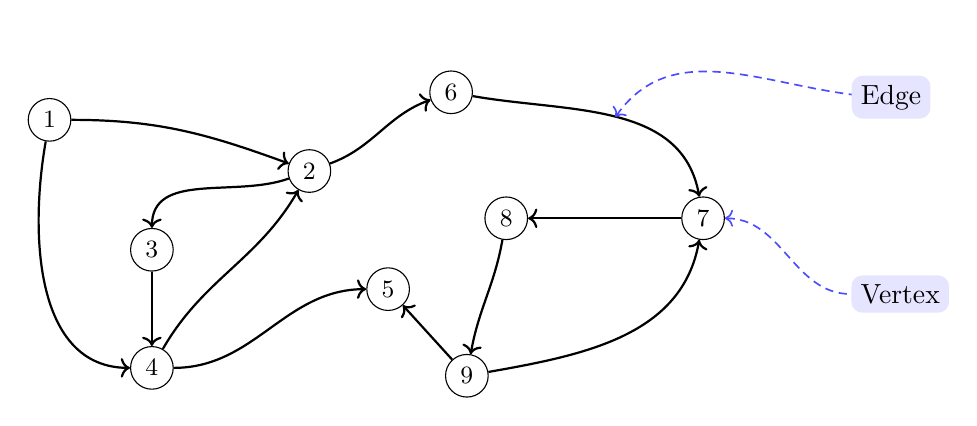
\begin{tikzpicture}[node/.style={draw, circle, inner sep=1mm}, edge/.style={->, thick}]

	\foreach \position [count=\count] in {(-1.3,.65), (2,0), (0,-1), (0,-2.5), (3,-1.5), (3.8,1), (7,-.6), (4.5,-.6), (4,-2.6)}
	{
		\node[node] (\count) at \position {\small \count};
	}

	\foreach \source/\target in {7/8, 9/5, 3/4} {
		\draw[->, thick] (\source) -- (\target);
	}

	\draw[edge] (1) to [in=180, out=-100] (4);
	\draw[edge] (1) to [in=160, out=0] (2);
	\draw[edge] (4) to [in=180, out=0] (5);
	\draw[edge] (6) to [in=100, out= -10] coordinate[midway] (e) (7);
	\draw[edge] (9) to [in=-100, out=10] (7);
	\draw[edge] (2) to [in=200, out=20] (6);
	\draw[edge] (8) to [in=80, out=-100] (9);
	\draw[edge] (4) to [in = -120, out=60] (2);
	\draw[edge] (2) to [in=90, out=-160] (3);

	\draw[densely dashed, <-, draw=blue!70, semithick] (e) to[out=55, in=180] +(3.5,.25) node[fill=blue!10, rounded corners] (Edge) {Edge};
	\node [below = 2.5 of Edge.west, anchor=west, fill=blue!10, rounded corners] (Vertex) {Vertex};
	\draw[densely dashed, <-, draw=blue!70, semithick] (7) to[out=0, in=180] (Vertex);

\end{tikzpicture}
\end{center}
\caption{A directed graph}%
\label{fig:graph-example}
\end{figure}

Graph partitioning algorithms partition a graph into equal sized subgraphs (in terms of nodes) in such a way that the number of edges cut is minimized. For example, Figure~\ref{fig:good-bad-partition} illustrates different ways of partitioning a graph, but not all alternatives provide an optimal solution. 

\begin{figure}[h]
\begin{center}
	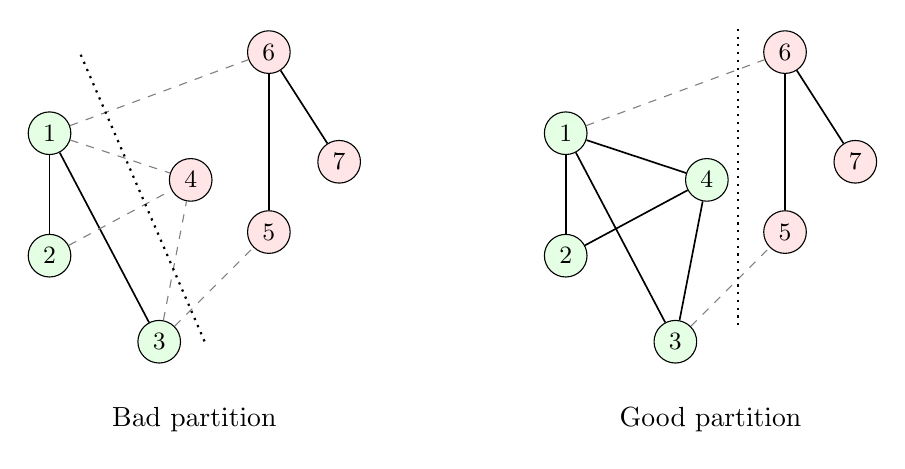
\begin{tikzpicture}[part1/.style={draw, circle, inner sep=1mm, fill=green!10},
		part2/.style={draw, circle, inner sep=1mm, fill=red!10},
		edge/.style={semithick}, cut/.style={dashed, gray}]

		\node[part1] (1-1) {\small 1};
		\node[part1, below = of 1-1] (1-2) {\small 2};
		\node[part1, below right = .7 and 1 of 1-2] (1-3) {\small 3};
		\node[part2, above right = of 1-3] (1-4) {\small 5};
		\node[part2, above right = .5 and .5 of 1-4] (1-5) {\small 7};
		\node[part2, above left = 1 and .5 of 1-5] (1-6) {\small 6};
		\node[part2, below right = 0.2 and 1.4 of 1-1] (1-7) {\small 4};

		\draw[cut] (1-1) -- (1-7);
		\draw[edge] (1-1) -- (1-2);
		\draw[edge] (1-1) -- (1-3);
		\draw[cut] (1-2) -- (1-7);
		\draw[cut] (1-3) -- (1-4);
		\draw[cut] (1-3) -- (1-7);
		\draw[edge] (1-4) -- (1-6);
		\draw[edge] (1-5) -- (1-6);
		\draw[cut] (1-1) -- (1-6);
		\coordinate[above right = .8 and .2 of 1-1] (c1);
		\coordinate[right = .3 of 1-3] (c2);

		\draw[dotted, thick] (c1) -- (c2);
		\coordinate (center1) at ($ (1-2)!.5!(1-5) $);
		\node[below = 2.4 of center1] {Bad partition};
		\node[part1,right = 6 of 1-1] (2-1) {\small 1};
		\node[part1, below = of 2-1] (2-2) {\small 2};
		\node[part1, below right = .7 and 1 of 2-2] (2-3) {\small 3};
		\node[part2, above right = of 2-3] (2-4) {\small 5};
		\node[part2, above right = .5 and .5 of 2-4] (2-5) {\small 7};
		\node[part2, above left = 1 and .5 of 2-5] (2-6) {\small 6};
		\node[part1, below right = 0.2 and 1.4 of 2-1] (2-7) {\small 4};

		\draw[edge] (2-1) -- (2-7);
		\draw[edge] (2-1) -- (2-2);
		\draw[edge] (2-1) -- (2-3);
		\draw[edge] (2-2) -- (2-7);
		\draw[cut] (2-3) -- (2-4);
		\draw[edge] (2-3) -- (2-7);
		\draw[edge] (2-4) -- (2-6);
		\draw[edge] (2-5) -- (2-6);
		\draw[cut] (2-1) -- (2-6);

		\coordinate[above left  = .1 and .4 of 2-6] (c3);
		\coordinate[below left  = 1 and .4 of 2-4] (c4);

		\draw[dotted, thick] (c3) -- (c4);
		\coordinate (center2) at ($ (2-2)!.5!(2-5) $);
		\node[below = 2.4 of center2] {Good partition};
\end{tikzpicture}
\end{center}
\caption{Different partitions of a graph}%
\label{fig:good-bad-partition}
\end{figure}



In the more general problem, edges can also have weights. Moreover, since this problem is a minimization problem, it can be modeled as an integer programming model, which is used commonly in operations research. 

\section{Project Planning}

The following is planned as follows:
\begin{enumerate}
	\item Construction of an integer programming model for the weightless, undirected graph partitioning problem.
	\item Development of an algorithm that solves the model using a integer programming solver like Gurobi.
	\item Construction of another model for the weighted version of the problem.
	\item Development of an algorithm for the weighted version of the problem.
	\item Evaluation of the software's performance in both cases (weighted and weightless) on a range of graph sizes and complexities.
\end{enumerate}

\subsection{Project Time and Resource Estimation}

The gantt chart for the project plan is in Figure~\ref{fig:project-plan}.

\begin{figure}[h]
\begin{center}
\begin{adjustbox}{max width=\textwidth}
\begin{ganttchart}[
hgrid,
vgrid,
time slot format=isodate,
bar label node/.append style={align=right},
y unit chart = 27mm,
y unit title = 17mm,
x unit = 3.6mm,
milestone/.append style={yscale=0.6, xscale=2.5, fill=YellowOrange, rounded corners=5pt},
bar/.append style={fill=SpringGreen!50, yscale=0.75},
]{2023-09-25}{2023-12-31}
\ganttset{bar height=.6}
\gantttitlecalendar{year, month=name, week} \\

%tasks
%project kickoff 20 Feb
\ganttmilestone{Project kickoff}{2023-09-27} \\
\ganttbar{Construction of an IP model\\for weightless, undirected\\graph partitioning problem}{2023-09-27}{2023-10-14} \\
\ganttbar{Software development for\\weightless, undirected\\graph partitioning problem}{2023-10-15}{2023-10-31} \\
\ganttbar{Evaluation of\\the performance of\\the software}{2023-11-01}{2023-11-15} \\
% midterm 3 apr
\ganttmilestone{Midterm report}{2023-11-19} \\
\ganttbar{Construction of model\\for the weighted version\\of the problem}{2023-11-20}{2023-11-30} \\
\ganttbar{Software development of\\the weighted version\\of the problem}{2023-12-01}{2023-12-14} \\
\ganttbar{Evaluation of the\\performance of the\\second software}{2023-12-15}{2023-12-26} \\
% end of classes: 26 dec
\ganttmilestone{End of classes}{2023-12-26}
\end{ganttchart}
\end{adjustbox}
\end{center}
\caption{Project Plan}
\label{fig:project-plan}
 \end{figure}
\subsection{Success Criteria}

The study is considered to be successful if

\begin{enumerate}
\item weightless and weighted graphs can be partitioned by software,
\item the software is able to partition large (but sparse) graphs. 
\end{enumerate}

\subsection{Risk Analysis}

\begin{enumerate}
	\item Technical Risks

		\begin{enumerate}
			\item Algorithm Complexity

				\begin{description}
					\item[Risk] The complexity of the algorithm may result in longer computation times, especially for larger graphs.
					\item [Impact] Delays in delivering results and potential resource strain.
					\item[Likelihood] High
					\item[Mitigation] Implement algorithm optimizations, explore parallel computing options, and conduct thorough testing on a range of graph sizes and densities.
				\end{description}

			\item Model Formulation Challenges

				\begin{description}
					\item[Risk] Difficulty in accurately formulating the graph partitioning problem as an IP model.
					\item[Impact] Incorrect solutions or failure to converge to an optimal solution.
					\item[Likelihood] Low
					\item[Mitigation] Perform rigorous testing on representative graph instances, conduct a comprehensive literature review.
				\end{description}
		\end{enumerate}

	\item Operational Risks

		\begin{enumerate}
			\item Resource Constraints

				\begin{description}
					\item[Risk] Inadequate computational resources for executing the algorithm efficiently.
					\item[Impact] Slower execution and potential limitations on the size of the graphs that can be processed.
					\item[Likelihood] Low to Moderate
					\item[Mitigation] Assess and secure sufficient computational resources, optimize code for resource efficiency, and maybe explore cloud computing options.
				\end{description}

			\item Data Security Concerns

				\begin{description}
					\item[Risk] Potential vulnerabilities in handling sensitive graph data.
					\item[Impact] Data breaches and/or unauthorized access.
					\item[Likelihood] Low
					\item[Mitigation] Implement secure data handling practices, use encryption where necessary.
				\end{description}
		\end{enumerate}
\end{enumerate}

\chapter{RELATED WORK}

The study of graph partitioning has a long history and can be traced back to various researchers and fields. While it's challenging to pinpoint a single origin, the problem has been explored by mathematicians, computer scientists, and researchers in related disciplines for many decades.

One early mention of graph partitioning can be found in the field of spectral graph theory. In the 1970s, researchers like F. R. K. Chung~\cite{chung1997spectral} began investigating the relationship between graph properties and eigenvalues of certain matrices associated with graphs. This work laid the foundation for spectral graph partitioning algorithms.

In the context of computer science and algorithms, the graph partitioning problem gained attention for parallel computing applications. During the 1980s and 1990s, researchers explored methods to efficiently partition graphs for parallel processing to optimize computational tasks. The proven NP-hard nature of the problem~\cite{feldmann} led researchers to develop heuristics as well as exact algorithms.

\section{Exact Algorithms}

A lot of research has been done on ways to solve the Generalized Partitioning Problem (GPP). Some methods are made specifically the bipartitioning case, while others work for the general GPP. Most of these methods use a common approach called the branch and bound framework.

Researchers use different strategies to set limits on the solutions. According to Buluç~\cite{buluc}, some use a method called semi-definite programming, like Karisch~\cite{karisch}, or Armbruster~\cite{armbruster}. Sellman and Sensen~\cite{sellmann, sensen} use something called multi-commodity flows. Linear programming is another technique used by Brunetta~\cite{brunetta}, Ferreira~\cite{ferreira}, Lisser~\cite{lisser}, and Armbruster~\cite{armbruster}, and others. Hager and others~\cite{hager13, hager99} take a continuous quadratic approach and then use the branch-and-bound method on it.

\section{Heuristics}

There are several heuristics proposed to solve graph partitioning problem.\\
Buluç~\cite{buluc} lists many heuristics, including:

\begin{itemize}
	\item Spectral Partitioning
	\item Graph Growing
	\item Flows
	\item Geometric Partitioning
	\item Streaming Graph Partitioning (SGP)
	\item Node-swapping Local Search
	\item Multilevel Graph Partitioning
\end{itemize}

\section{Graph Partitioning Software}

Several software packages implement various graph partitioning algorithms. Notable ones include:~\cite{buluc}


\begin{description}
  \item[Metis (and its variants kMetis and hMetis)] Known for its speed and flexibility, Metis is widely used for graph partitioning, with kMetis focusing on partitioning speed and hMetis emphasizing partition quality, especially in hypergraph scenarios.

  \item[Scotch] Developed by Pellegrini, Scotch offers a comprehensive graph partitioning framework with support for both sequential and parallel techniques. It utilizes recursive multilevel bisection for effective partitioning.

  \item[KaHIP (Karlsruhe High-Quality Partitioning)] Released by Sanders and Schulz, KaHIP implements various advanced methods, including flow-based techniques, more-localized local searches, and diverse parallel and sequential meta-heuristics. It has demonstrated high performance in challenges and benchmarks.

  \item[Chaco] One of the early publicly available packages, Chaco, developed by Hendrickson and Leland, implements multilevel approaches, basic local search algorithms, and spectral partitioning techniques.

  \item[ParMetis] A parallel implementation of the Metis GP algorithm by Karypis and Kumar, ParMetis is widely used for efficient graph partitioning in parallel computing environments.
\end{description}

\chapter{METHODOLOGY}

\section{Integer Programming}
Integer programming (IP) is a mathematical optimization technique used to find the optimal solution to a problem, where the decision variables are required to take integer values. It is a special case of linear programming (LP), where the decision variables can be any real number. In the context of graph partitioning, integer programming becomes a powerful tool for formulating and solving the problems. In our case, the goal is to find an optimal way to partition the graph's vertices while considering specific constraints, such as minimizing the number of edges between partitions.

\subsection{Methods of Solving Integer Programming Models}

\subsubsection{Branch and Bound}

Branch and bound is a common way of solving integer programming models. Before solving the problem, the integer constraints on decision variables are relaxed and treated as continuous variables. Then, a basic, feasible solution is found using regular linear programming solving techniques like the simplex method. If the basic solution contains originally integer variables that are fractional, then branch and bound algorithm starts.

For the variables that got fractional values, the problem is split into two branches by adding additional constraints to omit the fractional value from the set of feasible solutions: For example, if \( x_i \) is originally an integer variable but  \( x_i =5.3 \) in the relaxed LP formulation, one branch adds the constraint \( x_i \le 5 \) and the other adds \( x_i \ge 6 \). For each branch, the problem is solved again with the hope of finding an integer solution. This procedure is repeated until an integer solution is found and it is made sure that no better unknown solutions exist.~\cite{branch-bound} Figure~\ref{fig:branch-bound} summarizes the branch and bound method on a sample maximization problem with 2 integer variables (\( x_1, x_2 \)).

\begin{figure}[ht]
\begin{center}
	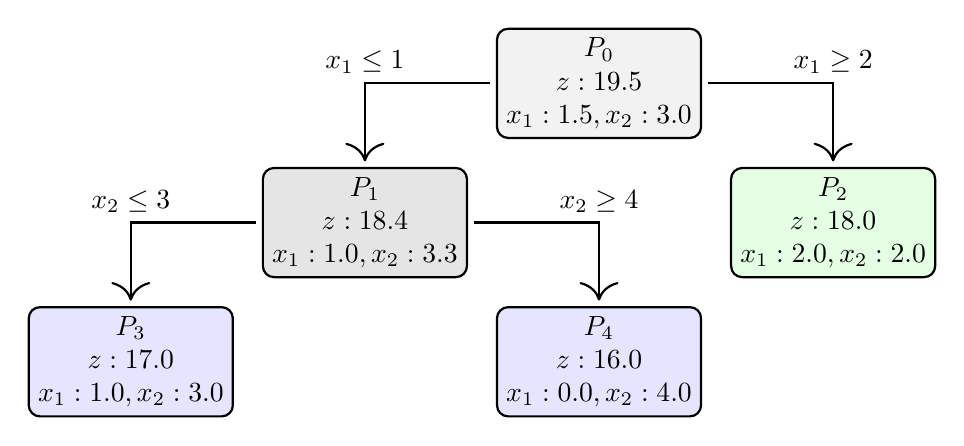
\begin{tikzpicture}[
		node/.style={draw, rectangle, rounded corners, align=center, thick},
		arrow/.style={arrows = {->[scale=2]},thick, shorten >= 2pt, shorten <= 2pt}]
	\node[node, fill=gray!10] (0) {\( P_0 \)\\ \( z: 19.5 \) \\ \( x_1: 1.5,  x_2: 3.0 \) };
	\node[node, below left = .5 of 0, fill=gray!20] (1) {\( P_1 \) \\ \( z: 18.4 \) \\ \( x_1: 1.0, x_2: 3.3 \)};
	\node[node, below right =.5  of 0, fill=green!10] (2) {\( P_2 \) \\ \( z: 18.0 \) \\ \( x_1: 2.0, x_2: 2.0 \)};
	\node[node, below left = .5 of 1, fill=blue!10] (3) {\( P_3 \) \\ \( z: 17.0 \) \\ \( x_1: 1.0, x_2: 3.0 \)};
	\node[node, below right = .5 of 1, fill=blue!10] (4) {\( P_4 \) \\ \( z: 16.0 \) \\ \( x_1: 0.0, x_2: 4.0 \)};

	\draw[arrow] (0) -| node[midway, above] {\( x_1 \le 1 \)}(1);
	\draw[arrow] (0) -| node[midway, above] {\( x_1 \ge 2 \)} (2);
	\draw[arrow] (1) -| node[midway, above] {\( x_2 \le 3 \)} (3);
	\draw[arrow] (1) -| node[midway, above] {\( x_2 \ge 4 \)} (4);
\end{tikzpicture}
\end{center}
\caption{Branch and bound method}%
\label{fig:branch-bound}
\end{figure}

\subsubsection{Cutting Plane}

Cutting plane method, is similar to branch and bound. Initially, the relaxed version of the problem is solved using simplex. (Integer constraints are discarded.) Then, if the solution includes variables violating the integer constraint, additional cutting constraints called ``Gomory cuts'' are added to tighten the relaxed problem. The Gomory cuts are special kinds of cuts in the feasible region of the problem that omit the previously found optimal (but violating integrality constraint) solution without eliminating any other integer solutions of the problem. Cuts are added iteratively to achieve an integer solution.~\cite{cutting-plane} An overview of the cutting plane algorithm can be seen in Figure~\ref{fig:cutting-plane}

\begin{figure}[ht]
\begin{center}
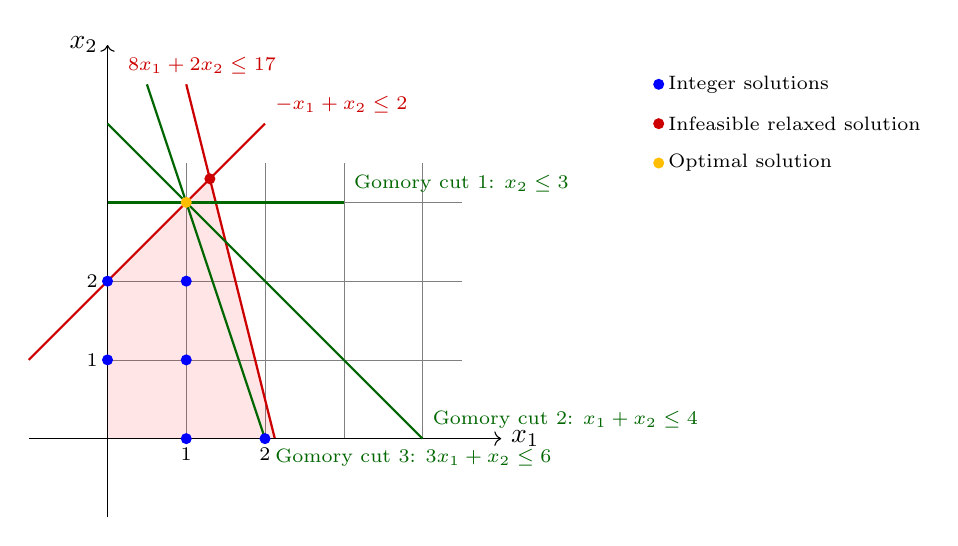
\begin{tikzpicture}[]
	\draw[step=1, ultra thin, gray] (0,0) grid (4.5,3.5);
	\fill[red, opacity = 0.1] (0,0) -- (0,2) -- (1.3,3.3) -- (17/8,0) -- cycle;
	\draw[->] (0,-1) -- (0,5) node[left] {\( x_2 \)};

	\draw[red!80!black, thick] (-1,1) -- (2,4) node[above right] {\scriptsize \( -x_1 + x_2 \le 2 \)};
	\draw[red!80!black, thick] (17/8,0) -- (1,4.5);
	\node [red!80!black, anchor=south] at (1.2,4.5) {\scriptsize \( 8x_1 + 2x_2 \le 17 \)};
	\draw[->] (-1,0) -- (5,0) node[right] {\( x_1 \)};
	\fill [red!80!black] (1.3, 3.3) circle (2pt);

	\draw[green!40!black, thick] (0,3) -- (3,3) node [above right] {\scriptsize Gomory cut 1: \( x_2 \le 3 \)};
	\draw[green!40!black, thick] (0,4) -- (4,0) node [above right] {\scriptsize Gomory cut 2: \( x_1 + x_2 \le 4 \)};
	
	\draw[green!40!black, thick] (0.5,4.5) -- (2,0) node [below right] {\scriptsize Gomory cut 3: \( 3x_1 + x_2 \le 6 \)};

	\foreach \x in {1,2} {
		\fill[blue] (\x,0) circle (2pt) node [below, black] {\scriptsize \x};
	}
	\foreach \y in {1,2} {
		\fill[blue] (0, \y) circle (2pt) node [left, black] {\scriptsize \y};
	}
	\foreach \position in {(1,1), (1,2)} {
		\fill[blue] \position circle (2pt);
	}
	\fill[orange!50!yellow] (1,3) circle (2pt);

	\fill[blue] (7,4.5) circle (2pt) node [right, black] {\scriptsize Integer solutions};
	\fill [red!80!black] (7,4) circle (2pt) node [right, black] {\scriptsize Infeasible relaxed solution};
	\fill[orange!50!yellow] (7,3.5) circle (2pt) node [right, black] {\scriptsize Optimal solution};
\end{tikzpicture}
\end{center}
\caption{Cutting plane method}%
\label{fig:cutting-plane}
\end{figure}

\section{Gurobi}

Gurobi is a cutting-edge optimization engine designed for solving complex mathematical optimization problems, including integer programming.~\cite{gurobi} Gurobi uses branch and bound and cutting plane methods together while solving an integer model, and the joint use of these methods is called ``branch and cut''. One of Gurobi's notable features is its ability to perform parallel optimization, harnessing the power of modern computing architectures to accelerate problem-solving. By efficiently distributing computation across multiple processors, Gurobi enhances the speed and scalability of integer programming solutions. Because of these reasons, Gurobi is utilized in the software.

\chapter{REQUIREMENTS SPECIFICATION}

\begin{enumerate}
	\item Functional Requirements
		\begin{enumerate}
			\item Algorithm
				\begin{enumerate}
					\item The algorithm \must\ partition the graph into two equal subgraphs with minimum edge cuts.
					\item The algorithm \must\ be able to receive a graph from the user as input.
					\item The algorithm \must\ be able to give the output of edges cut and the partition information back to the user.
				\end{enumerate}

			\item Implementation
				\begin{enumerate}
					\item The algorithm \must\ use the methodologies for solving integer programming models.
					\item The software \shall\ utilize integer programming model solvers like Gurobi, CPLEX when solving the IP model.
				\end{enumerate}
			\item Performance
				\begin{enumerate}
					\item The software \must\ be able to partition graphs of different sizes and densities.
				\end{enumerate}
		\end{enumerate}

\end{enumerate}


\chapter{DESIGN}

\section{Information Structure}

The software is not linked to any database management system. The information flow occurs with basic input and output files and the terminal.


\subsection{Input}

\subsubsection{Graph Data}
The input graph is taken from the user and must be in the form of a Matrix Market file (.mtx file). The Matrix Market (MM) exchange formats is an ASCII based, human readable format designed by NIST\footnote{National Institute of Standards and Technology} as a convenient way of exchanging matrix data.~\cite{matrix-market} The input matrix provided by the user has to be a symmetric matrix, as the software can only parititon undirected graphs.

\subsection{Output}
\subsubsection{Gurobi's Log}
The user can provide a log file name as an option when running the program in the terminal to tell Gurobi to write logs. The log file is a human readable, simple, text file that includes details about the optimization process of Gurobi.

\subsubsection{Graph Plots}
The user can provide a flag when running the program in the terminal to tell the software to draw a plot of the graph with the partitions.

\subsubsection{Graph Partitioning Data}

After a graph is partitioned, the user receives the graph partitioning data (edges cut, clusters etc.) from the terminal.


\section{Information Flow}

The flow of the software is summarized in Figure~\ref{fig:sequence-diagram}.
\begin{figure}[ht]
	\centering
	\begin{sequencediagram}
	\newthread{u}{User}
	\newinst[2.5]{p}{Graph Partitioner}
	\newinst[2.5]{g}{Gurobi Engine}
	\begin{call}{u}{Undirected Graph}{p}{Graph partitioning info}
		\begin{call}{p}{\texttt{readInput()}}{p}{\texttt{adjacencyMatrix}}
		\end{call}
		\postlevel
		\begin{call}{p}{\texttt{buildGurobiModel()}}{p}{\texttt{model}}
		\end{call}
		\postlevel
		\begin{call}{p}{\texttt{model.optimize()}}{g}{Graph partitioning info}
		\end{call}
	\end{call}
	\end{sequencediagram}
	\caption{Sequence Diagram}
	\label{fig:sequence-diagram}
\end{figure}

\section{System Design}

\subsection{Integer Programming Model}

Let's define \( V = \left\{ 1,\dots,n \right\} \) as the set of vertices in the graph, and \( W \) as the adjacency matrix of the graph, which can be both weighted and weightless. \( w_{ij} \neq 0 \) if there is an edge from vertex \( i \) to \( j \), and 0 otherwise. For each vertex \( i \in V\), we need to determine the node's partition. We name the partitions as 
partition \#0 and partition \#1 for convenience.

Since the graph partitioning problem is a minimization problem, we can model it as an Integer Programming model. Our goal is to minimize the sum of the penalties attained for each edge cut. When the graph is weightless, penalties associated with cutting each edge is equal and equal to 1. On the other hand, if the graph is weighted, the each penalty for cutting an edge is the weight of that edge.

The first thing that should be done when building an Integer Programming model is to decide on the decision variables. In this problem, for each edge from vertex \(i\) to \(j\), we need to decide whether to cut it or not. For each \( i,j \in V\) and \( w_{ij} \neq 0 \), we define \( x_{ij} \) as a decision variable that is 1 if an edge will be cut between \( i \) and \( j \), and 0 otherwise. The variable is defined only when \( w_{ij} \neq 0 \) because the edge \(i\) to \(j\) must be present before actually cutting it. Moreover, we need to decide on the partition of each vertex. We can denote the partition of vertex \( i \) as \( p_i \). \( p_i \) can be either 0 or 1

On top of these, it is worth mentioning that we will use only the lower triangle of the adjacency matrix because the adjacency matrix is symmetric, and using only one half of the matrix is enough to build the model.

The objective function of this problem will be the sum of all \( w_{ij} \times x_{ij} \)'s.

\subsubsection{Sets}

\begin{itemize}
	\item \( V = \left\{ 1,\dots,n \right\}  \): the set of vertices.
\end{itemize}

\subsubsection{Parameters}
\begin{itemize}
	\item \( w_{ij} = \begin{cases}
			>0, & \text{if vertex $i$ and $j$ are connected} \\
			0, &  \text{if vertex $i$ and $j$ are not connected}
	\end{cases} , \forall i,j \in V, i<j\)
\end{itemize}

\subsubsection{Decision Variables}
\begin{itemize}
	\item \( x_{ij} = \begin{cases}
		1, &\text{\small  if the edge between vertex \( i \) and \( j \) is ``cut''}\\
		0, & \text{\small the edge is not touched, vertex \( i \) and \( j \) are connected}
	\end{cases} , \forall i,j \in V, w_{ij} \neq 0\)
	\item \( p_i = \begin{cases}
		1, &\text{ if vertex \( i \) is in partition \#1}\\
		0, & \text{if vertex \( i \) is in partition \#0}
	\end{cases}, \forall i \in V \)
\end{itemize}

\subsubsection{Objective Function}
\begin{itemize}
	\item minimize \( \displaystyle\sum_{i=2}^{n} \displaystyle\sum_{j\in V | w_{ij} \neq 0} w_{ij} \times x_{ij} \)
\end{itemize}

In order for this model to work, we have to define the constraints of a model:

\begin{enumerate}
	\item If nodes \( i \) and \( j \) are connected (if \(x_{ij} = 0\)), they have to be in the same partition. (\( p_i = p_j \))
	\item Partition sizes must be equal.
\end{enumerate}

So, with everything set, here is the summary of our integer programming model:

\begin{mini*}[1]
	{}{\sum_{i=2}^{n} \sum_{j\in V | w_{ij} \neq 0} w_{ij} \times x_{ij}}
{\label{eq:IPmodel}}{}
\addConstraint{p_i - p_j}{\le x_{ij}}{\hspace{1cm} \forall i,j \in V, w_{ij} \neq 0, \text{ (Adjacent nodes are in the same partition)}}
\addConstraint{p_i - p_j}{\ge -  x_{ij}}{\hspace{1cm}\forall i,j \in V, w_{ij} \neq 0, \text{ (Adjacent nodes are in the same partition)}}
\addConstraint{\sum_{i=1}^{n} p_i}{= \left \lfloor \frac{n}{2}  \right \rfloor }{\hspace{1cm}\text{(Equal partition sizes)}}
\addConstraint{x_{ij}}{=\left\{ 0,1 \right\} }{\hspace{1cm}\forall i,j \in V, w_{ij} \neq 0, \text{ (Binary variable constraint)}}
\addConstraint{p_i}{=\left\{ 0,1 \right\}}{\hspace{1cm}\forall i \in V, \text{ (Binary variable constraint)}}
\end{mini*}


\chapter{IMPLEMENTATION AND TESTING}

\section{Implementation}

The integer programming model for the weightless graph partitioning is programmed in Python using Gurobi's Python API (\texttt{gurobipy} library). Python is preferred in this project because of its ease of use, support for Matrix Market File (.mtx file) I/O using \texttt{scipy} library, and the availability of great graph visualization tools with the help of \texttt{igraph} and \texttt{matplotlib} libraries.\\
The repository of the software can be obtained from~\cite{dortogul}.

\section{Testing}

The performance of the program is tested with various graphs on a MacBook Pro with the following hardware:

\begin{description}
	\item[Processor Name] Quad-Core Intel Core i5
	\item[Processor Speed] 1.4GHz
	\item[Number of Processors]: 1
	\item[Total Number of Cores]: 4
	\item[L2 Cache (per Core)] 256 KB
	\item[L3 Cache] 6 MB
	\item[Hyper-Threading Technology] Enabled
	\item[Memory] 16 GB
\end{description}

The results of the test is discussed in Section~\ref{sec:results}.

\section{Deployment}

To be able to run the program, the user should obtain a license from Gurobi's website, which is free for academic use. After installing the license in a computer, the program's repository can be cloned with the following command:

\noindent \texttt{git clone}\\
{\small \url{https://github.com/araldortogul/CMPE492_Partitioning_Undirected_Graphs.git}}

The required Python libraries are listed in \texttt{requirements.txt}, and they can be downloaded by typing the command:

\noindent \texttt{pip install -r requirements.txt}

\noindent inside the project repository.

After cloning, the program can be run by opening a terminal in the repository and typing

\texttt{./graph\_partitioner.py}

\noindent Here is the usage of \texttt{graph\_partitioner}:


\lstinputlisting{usage.txt}

\chapter{RESULTS}
\label{sec:results}


\section{Small, Weighted Graphs}

The software is able to partition weighted, small graphs (size between 20 and 30) very quickly. According to the average runtimes in Figure~\ref{fig:p1}, higher density results in higher computation time. This is expected because the IP model has \( |V| + |E| \) decision variables and \( 1 + |V| + 3 \times |E| \) constraints.

\begin{figure}[ht]
	\centering
	\includesvg{p1}
	\caption{Runtimes of Small, Weighted Graphs with Different Densities}
	\label{fig:p1}
\end{figure}

\section{Small, Weightless Graphs}

The software is also able to partition weightless, small graphs of all densities in reasonable time. However, unlike the weighted version, high density does not always lead to high runtime. According to the runtimes in Figure~\ref{fig:p2}, densities 0.6 and 0.7 took the most time to find the best solution. This may be due to the fact that very dense graphs (density \(>\) 0.8) might be predictable in terms of the number of cuts. On the contrary, in the weighted version of the problem, the weights of the individual edges have a significant impact on the outcome, so the edges should be handled more carefully in the weighted version.

\begin{figure}[ht]
	\centering
	\includesvg{p2}
	\caption{Runtimes of Small, Weightless Graphs with Different Densities}
	\label{fig:p2}
\end{figure}

\section{Graph between 50 and 100 Vertices}

Dense graphs with more than 50 vertices become too complex for the software to find a solution quickly. The software is tested on sparse graphs between 75 and 100 vertices, and Figure~\ref{fig:p4} and Figure~\ref{fig:p5} display the runtimes for the weighted and weightless versions of the problem. 

\begin{figure}[ht]
	\centering
	\includesvg{p4}
	\caption{Runtimes of Weighted, Sparse Graphs between 75 and 100 Vertices}
	\label{fig:p4}
\end{figure}

\begin{figure}[ht]
	\centering
	\includesvg{p5}
\caption{Runtimes of Weightless, Sparse Graphs between 75 and 100 Vertices}
	\label{fig:p5}
\end{figure}

One major finding from the data in Figure~\ref{fig:p4} and Figure\ref{fig:p5} is that the weightless version of the problem takes slighlty more time to find a solution than the weighted version.

\section{Large, Sparse Graphs}

For large graphs (size \(>\) 100), the software is tested on very low densities. Figure~\ref{fig:p3} shows how the average runtime of the algorithm changes when the graph size increases for densities 0.01, 0.02 and 0.03. Graphs with 0.03 density can be solved under 1 minute if the size of the graph is less than 150. Graphs with 0.02 density are slightly easier to solve, and the computation takes less than 1 minute for sizes less than 180. Finally, graphs with 0.01 density can be solved up to size 250.

\begin{figure}[H]
	\centering
	\includesvg{p3}
	\caption{Runtimes of Large, Sparse Graphs with Different Densities}
	\label{fig:p3}
\end{figure}


\section{Sample Graphs and their Partitions}

\subsection{Graphs from SuitSparse Matrix Collection}

In this section, sample sparse matrices are taken from SuiteSparse Matrix Collection~\cite{sparse-collection}. 

Here are some examples of solved cases:

\subsubsection{Graph 1}

\begin{itemize}
	\item Name: Pajek/GD96\_c
	\item Description: Pajek network: Graph Drawing contest 1996
	\item Size: 65
	\item Edges: 250
\end{itemize}


\begin{figure}[H]
    \centering
    \begin{minipage}{.5\textwidth}
        \centering
	\includegraphics[width=.9\linewidth]{GD96_c-adjacency}
        \caption{Adjacency Matrix of GD96\_c}
        \label{fig:adjacency-1}
    \end{minipage}%
    \begin{minipage}{0.5\textwidth}
        \centering
	\includesvg[width=.9\linewidth]{GD96_c}
        \caption{Solution for GD96\_c}
        \label{fig:sol1}
    \end{minipage}
\end{figure} 

\subsubsection{Graph 2}
\begin{itemize}
	\item Name: HB/dwt\_59
	\item Description: Symmetric Connection Table from Dtnsrdc, Washington
	\item Size: 59
	\item Edges: 267
\end{itemize}

\begin{figure}[H]
    \centering
    \begin{minipage}{.5\textwidth}
        \centering
	\includegraphics[width=.9\linewidth]{dwt_59-adjacency}
        \caption{Adjacency Matrix of dwt\_59}
        \label{fig:adjacency-2}
    \end{minipage}%
    \begin{minipage}{0.5\textwidth}
        \centering
	\includesvg[width=.9\linewidth]{dwt_59}
        \caption{Solution for dwt\_59}
        \label{fig:sol2}
    \end{minipage}
\end{figure}

\subsection{Weightless Erdős–Rényi Graphs}

Here are some example solutions for weightless random graphs generated by the Erdős–Rényi model.

\begin{figure}[H]
    \centering
    \begin{minipage}{.5\textwidth}
        \centering
	\includesvg[width=.9\linewidth]{erdos-1}
    \end{minipage}%
    \begin{minipage}{0.5\textwidth}
        \centering
	\includesvg[width=.9\linewidth]{erdos-2}
    \end{minipage}
\caption{Solutions of Randomly Generated Weightless Graphs}
\end{figure}

\subsection{Weighted Erdős–Rényi Graphs}

Here are some example weighted random graphs generated by the Erdős–Rényi model. Weights of the edges are uniformly distributed between 1 and 5.

In the plots, edges with higher weghts are drawn thicker.

\begin{figure}[H]
    \centering
    \begin{minipage}{.5\textwidth}
        \centering
	\includesvg[width=.9\linewidth]{erdos-3}
    \end{minipage}%
    \begin{minipage}{0.5\textwidth}
        \centering
	\includesvg[width=.9\linewidth]{erdos-4}
    \end{minipage}
\caption{Solutions of Randomly Generated Weighted Graphs}
\end{figure}

\chapter{CONCLUSION}

The integer programming model developed for the graph partitioning problem can handle the bipartitioning of small graphs and sparse, large graphs. It gives promising results and can be further improved by generalizing the problem to partitioning the graph into more than 2 subgraphs. The program may be used for partitioning data that is sparsely connected. 

This project helped me refine my operations research knowledge as well as my software developing skills. Moreover, it shows how approaching in an interdisciplinary fashion helps finding unique solutions to engineering problems.

\bibliographystyle{styles/fbe_tez_v11}
\bibliography{references}

\appendix	


\end{document}
